\documentclass[12pt,a4paper]{article}
\usepackage{float}
\usepackage{commands}
\usepackage{indentfirst}

\title{
	\Huge{\bf{Report for Assignment 3}}
}
% \author{
% NAME \\
% 	\texttt{EMAIL} \\
% 	STUDENT NUMBER
% }
\date{
\today
}


\begin{document}
\maketitle
\section{Implementation}

Based on the code given, we implement the path planning simulation domain (2D map navigation) in \textbf{createDomain.py}. We treat the domain as an object which consists of its dimension, obstacles, goal and start. When creating a domain instance, we specify the number of obstacles and the maximum size of the obstacles, which helps facilitate our experiment in part 4. We also write some codes to help visualize our result by using matplotlib.pyplot. This function, whose name is \textbf{drawDomain}, receives a path (a list of tuples) and draws the path within the domain. Optionally, it can take a list of the nodes generated by the state space 
partitioning. 

\subsection{Quadtree and FBSP Decomposition}

We first created a Quadrant object in \textbf{quad.py}.
This object represents a quadrant. It is capable of
returning if it is entirely an obstacle, entirely empty
space or mixed. It is also capable of spliting itself
into four smaller Quadrant object.\\

Then we simply implement Quadtree Decomposition by setting the first quadrant to as the entire domain, and 
recursivly splitting it down into smaller objects until 
we are left with no mixed quadrants. This is done
in \textbf{decompose.py}.\\

Then we implement a State object, in \textbf{decompose.py}, 
that takes a list of full Quadrants and a list of empty
Quadrants. It generates a set of nodes for our searching
algorithm to search through. Instead of having a node at
the center of each quadrant, we have a node at the center 
of each wall shared by two quadrants. This eliminates the
algorithms tendency to find paths that go straight over
corners.\\

Finally, a basic A* search is implmented in \textbf{a\_star.py}.\\

For FBSP Decomposition, we use scikit-learn's decision tree classifier with entropy as a loss function. We train 
a tree on each of the coordinates as the feature and 
whether its empty or not as the label. We then convert
the decision boundry at each leaf of the tree into our
Quadrant object. This is done in \textbf{decompose.py}. After this we can procceed exacty as we did for QTD.

\subsection{Rapidly Exploring Random Tree (RRT)}
We first implement some additional data structures (Node and Tree) in \textbf{Structure.py}. Node is a subclass of obstacle but it has one more instance: parent. Each tree consists of a list of nodes and its root. Each tree has a function called \textbf{findNearestNode}, it receives a node in the domain and outputs the nearest node in the tree.\\

We then implement the algorithm in \textbf{RRTsolver.py}. A solver receives a problem instance (a domain) and outputs the solution and stats. At each iteration, \textbf{solve} (the algorithm) generates a random node with some probability of choosing the goal(\textbf{randomNode}). Then it attempts to find a new node on the line connecting the random node and the nearest node, determined by the step size. Finally, it connect this new node to the nearest node in the tree (\textbf{extend}). When the new node is extremely close to the goal, the algorithm connects the new node and the goal directly and the problem is solved and \textbf{traceBack} is triggered. It takes advantage of the data structure and outputs a whole path from the goal to the start by calling a node's parent repeatedly. 

\section{Results}
\subsection{Quadtree vs FBSP Decomposition}

Below are figures of the solution found for different
domain types. The first row is the domain, the second is the QTD's solution
and the third is the FBSP's solution.\\

\newpage

10 obstacles with length,width$\sim$ uniform$(10,20)$\\
\begin{figure}[H]
\centering
	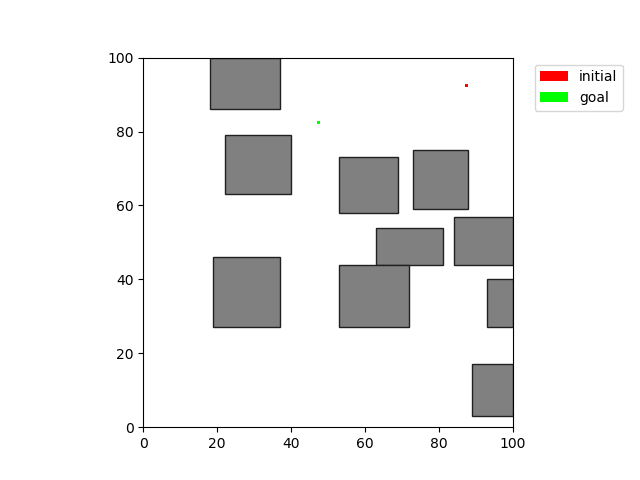
\includegraphics[scale=.40]{10_20_emp}
\caption{Domain}
\end{figure}

\begin{figure}[H]
\centering
	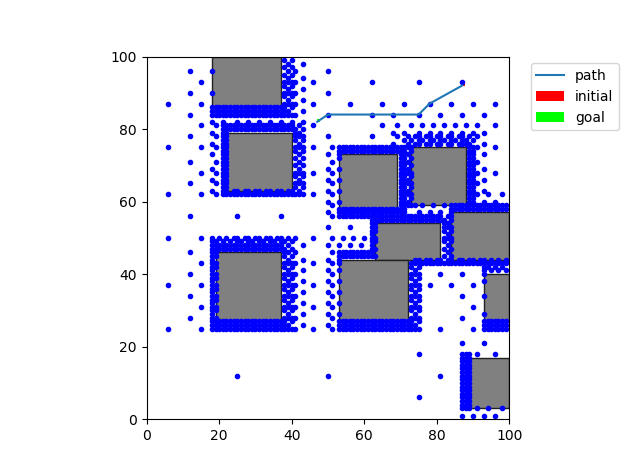
\includegraphics[scale=.40]{10_20_qtd_state}
    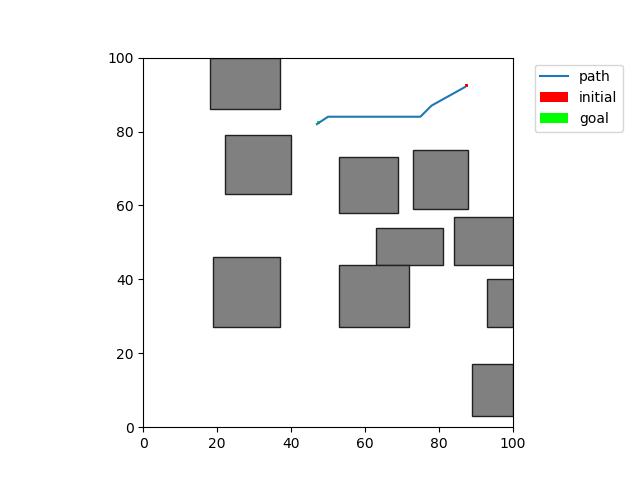
\includegraphics[scale=.40]{10_20_qtd_path}
\caption{QTD}
\end{figure}

\begin{figure}[H]
\centering
	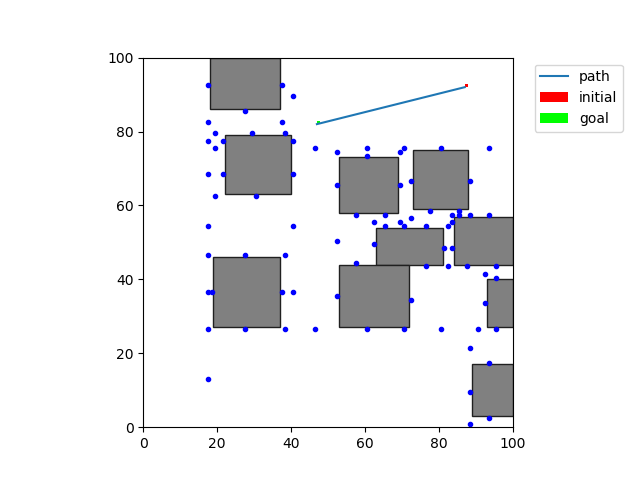
\includegraphics[scale=.40]{10_20_fbsp_state}
    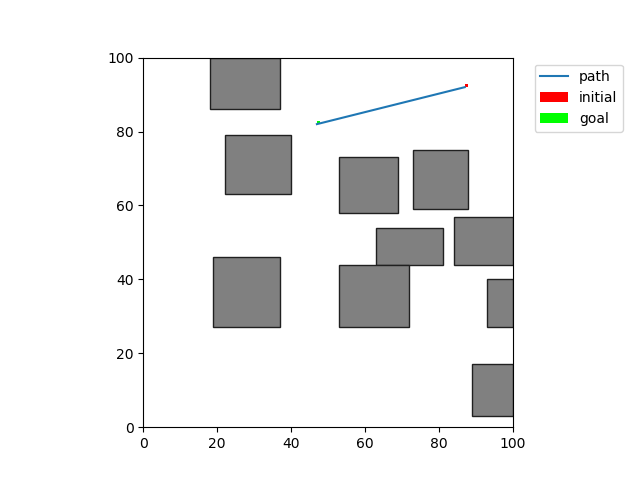
\includegraphics[scale=.40]{10_20_fbsp_path}
\caption{FBSP}
\end{figure}

\newpage

10 obstacles with length,width$\sim$ uniform$(10,50)$\\
\begin{figure}[H]
\centering
	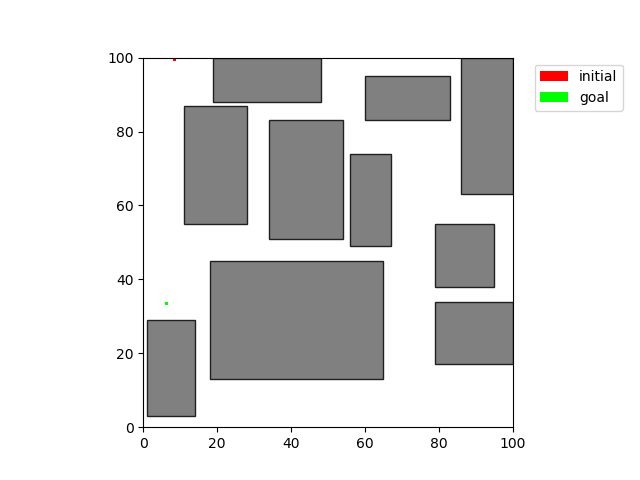
\includegraphics[scale=.40]{10_50_emp}
\caption{Domain}
\end{figure}

\begin{figure}[H]
\centering
	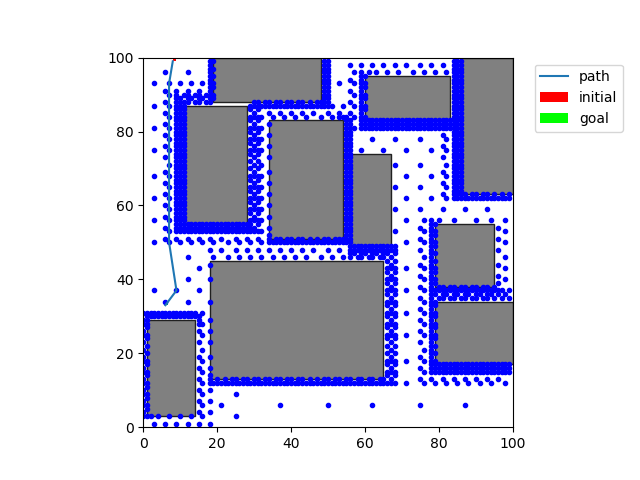
\includegraphics[scale=.40]{10_50_qtd_state}
    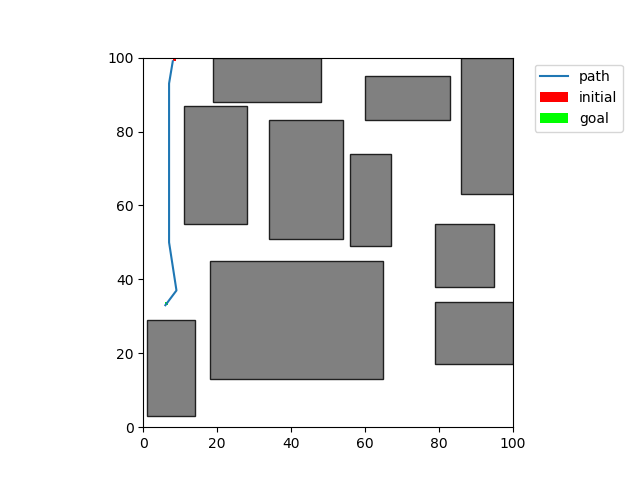
\includegraphics[scale=.40]{10_50_qtd_path}
\caption{QTD}
\end{figure}

\begin{figure}[H]
\centering
	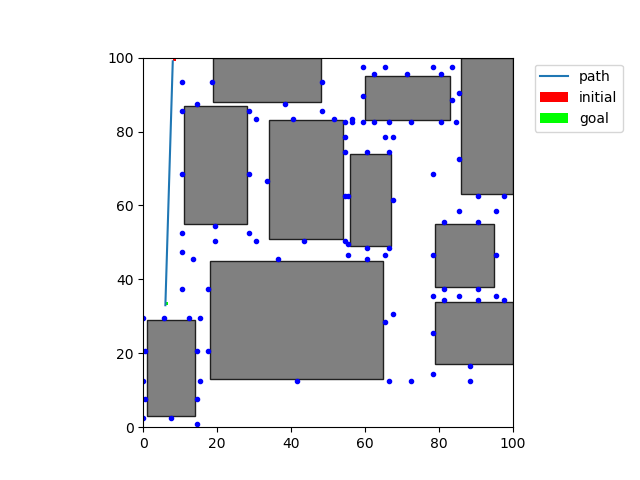
\includegraphics[scale=.40]{10_50_fbsp_state}
    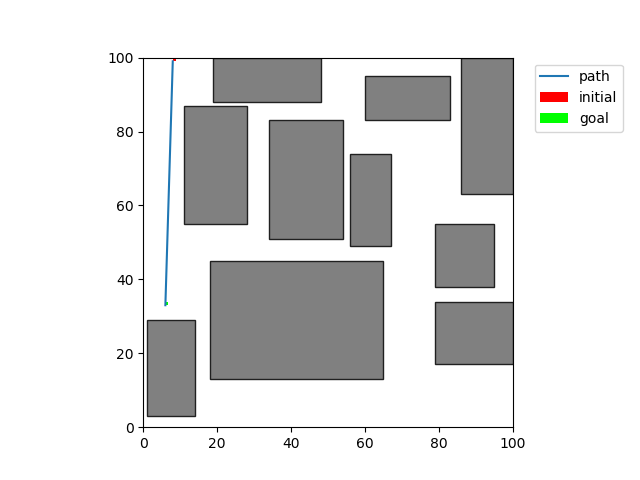
\includegraphics[scale=.40]{10_50_fbsp_path}
\caption{FBSP}
\end{figure}

\newpage

20 obstacles with length,width$\sim$ uniform$(10,20)$\\
\begin{figure}[H]
\centering
	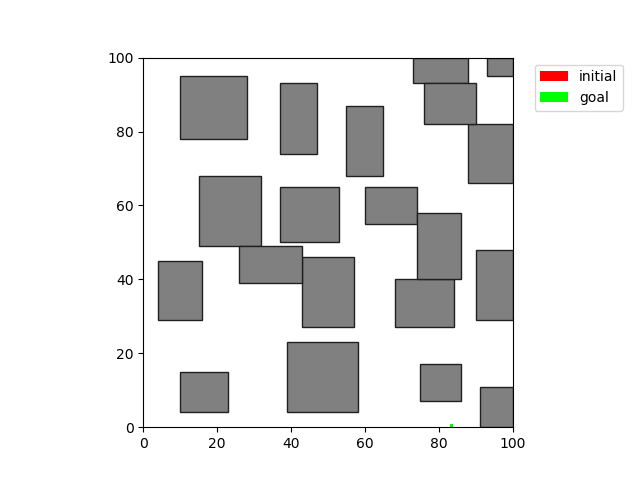
\includegraphics[scale=.40]{20_20_emp}
\caption{Domain}
\end{figure}

\begin{figure}[H]
\centering
	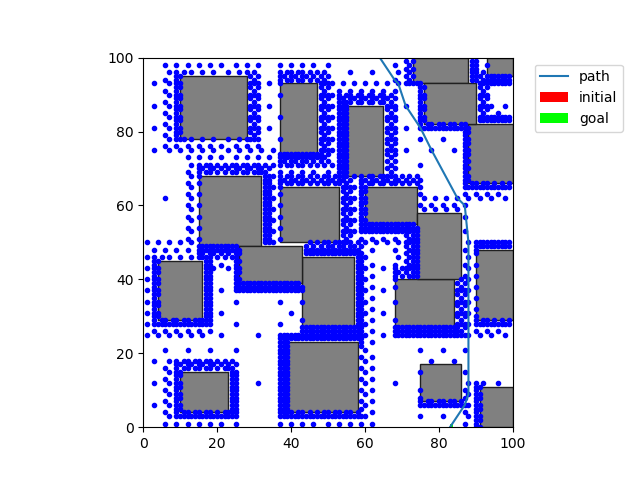
\includegraphics[scale=.40]{20_20_qtd_state}
    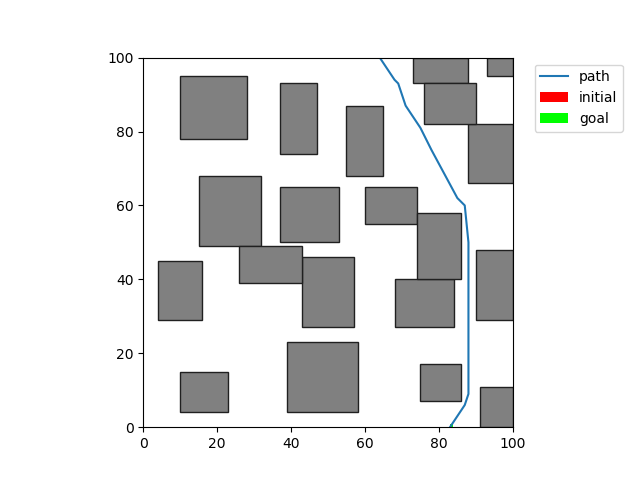
\includegraphics[scale=.40]{20_20_qtd_path}
\caption{QTD}
\end{figure}

\begin{figure}[H]
\centering
	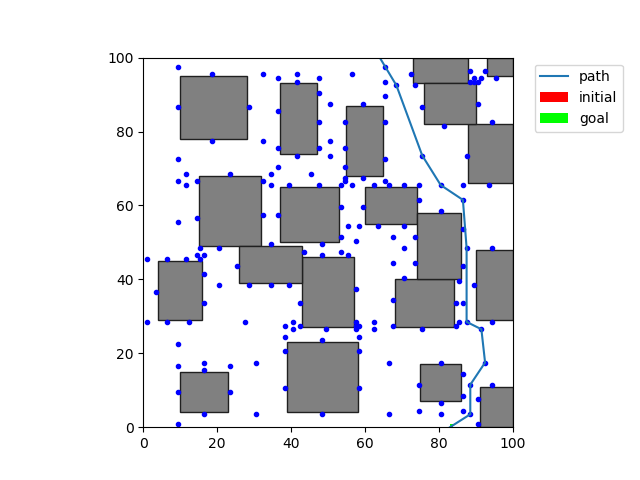
\includegraphics[scale=.40]{20_20_fbsp_state}
    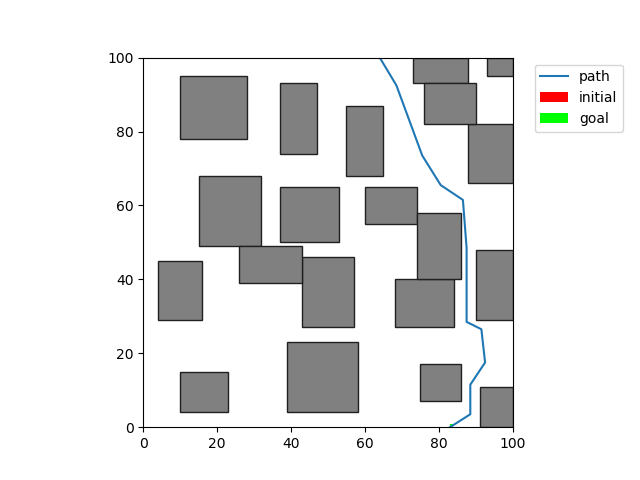
\includegraphics[scale=.40]{20_20_fbsp_path}
\caption{FBSP}
\end{figure}

\newpage

20 obstacles with length,width$\sim$ uniform$(10,50)$\\
\begin{figure}[H]
\centering
	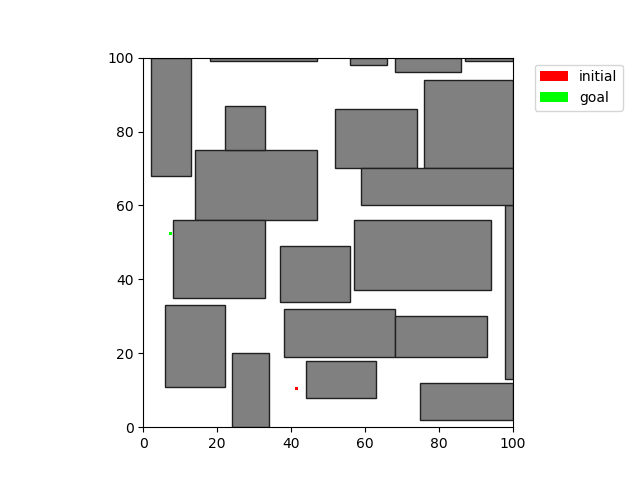
\includegraphics[scale=.40]{20_50_emp}
\caption{Domain}
\end{figure}

\begin{figure}[H]
\centering
	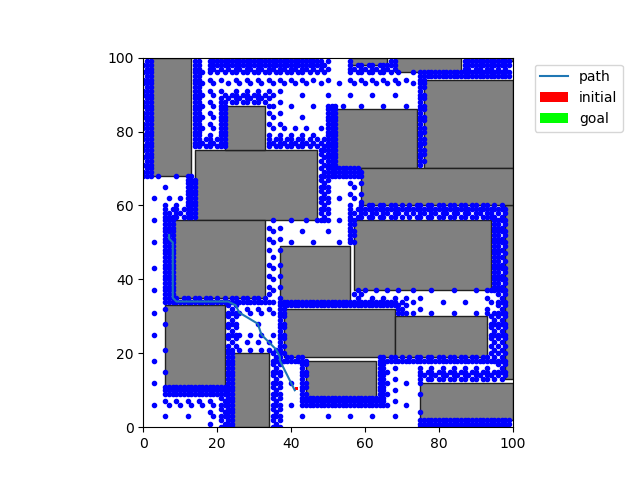
\includegraphics[scale=.40]{20_50_qtd_state}
    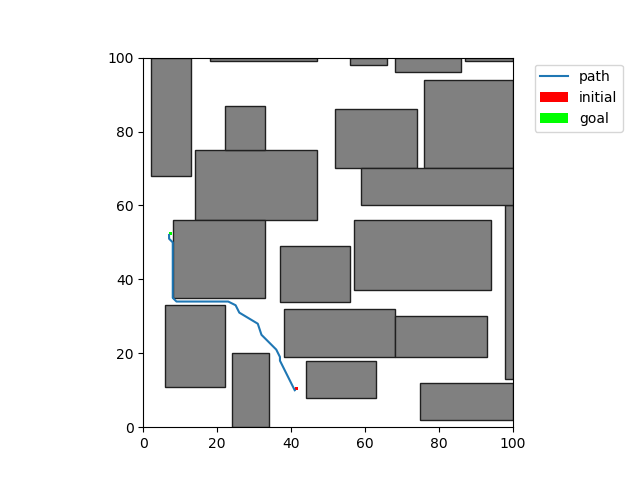
\includegraphics[scale=.40]{20_50_qtd_path}
\caption{QTD}
\end{figure}

\begin{figure}[H]
\centering
	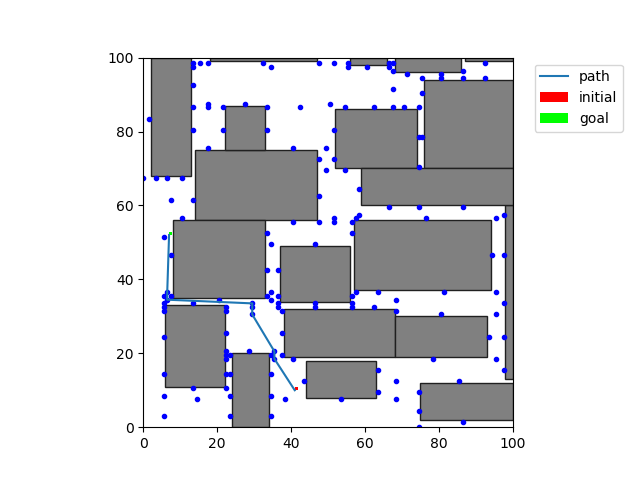
\includegraphics[scale=.40]{20_50_fbsp_state}
    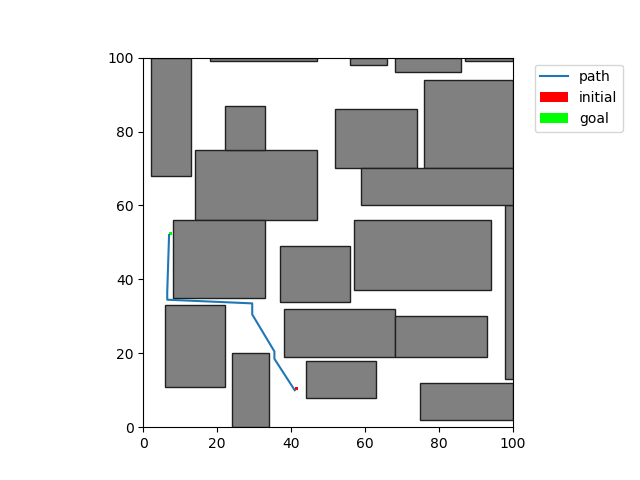
\includegraphics[scale=.40]{20_50_fbsp_path}
\caption{FBSP}
\end{figure}

\newpage

30 obstacles with length,width$\sim$ uniform$(10,20)$\\
\begin{figure}[H]
\centering
	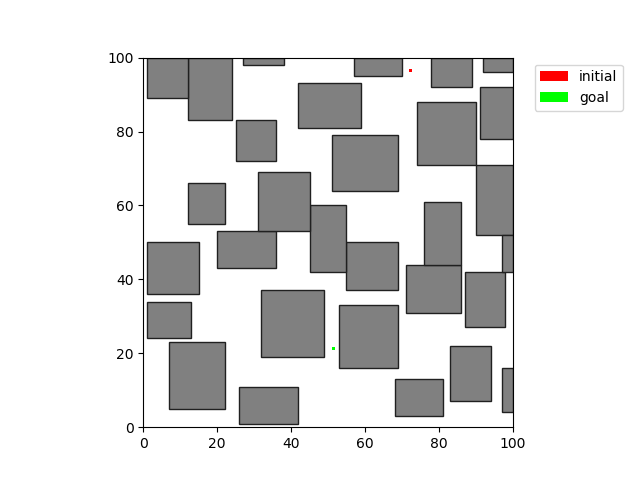
\includegraphics[scale=.40]{30_20_emp}
\caption{Domain}
\end{figure}

\begin{figure}[H]
\centering
	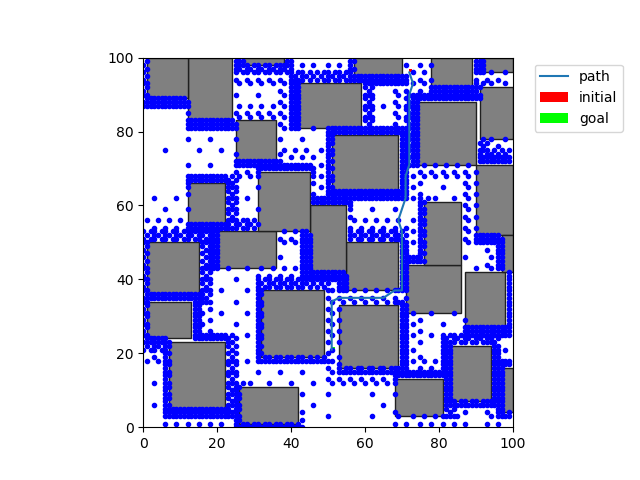
\includegraphics[scale=.40]{30_20_qtd_state}
    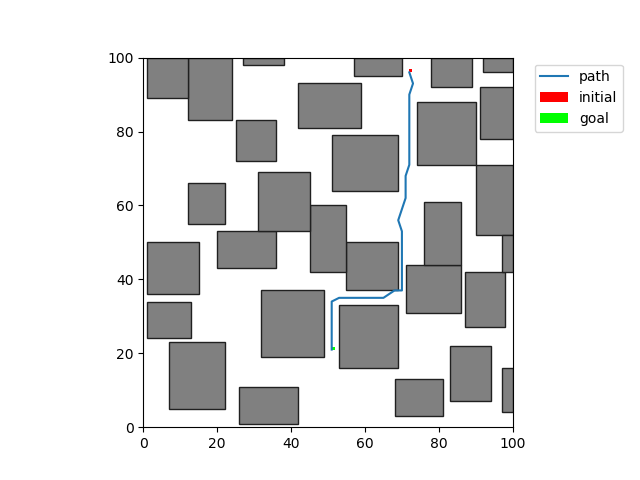
\includegraphics[scale=.40]{30_20_qtd_path}
\caption{QTD}
\end{figure}

\begin{figure}[H]
\centering
	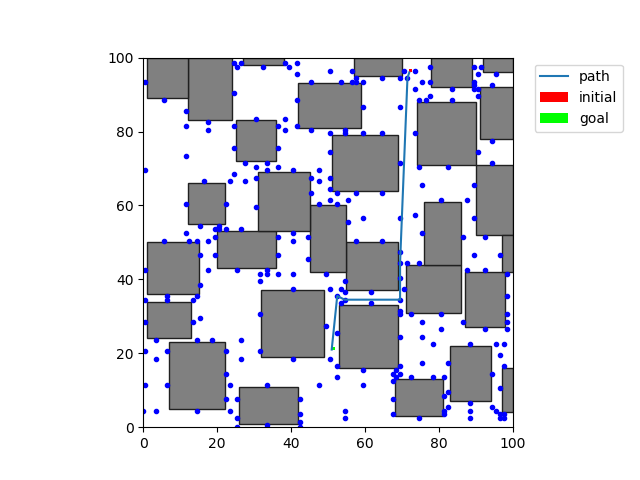
\includegraphics[scale=.40]{30_20_fbsp_state}
    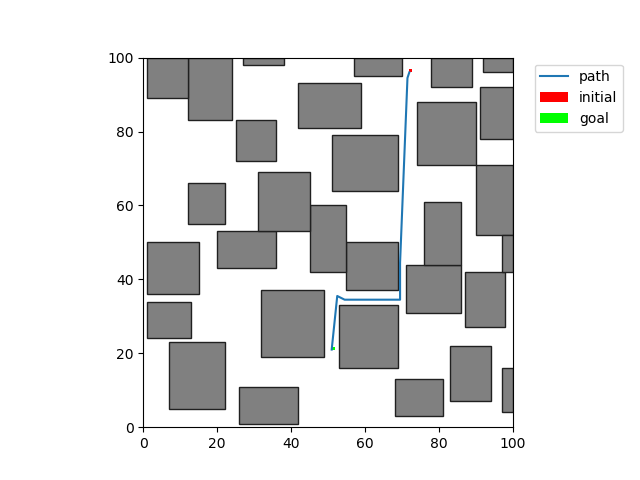
\includegraphics[scale=.40]{30_20_fbsp_path}
\caption{FBSP}
\end{figure}

\newpage

40 obstacles with length,width$\sim$ uniform$(10,20)$\\
\begin{figure}[H]
\centering
	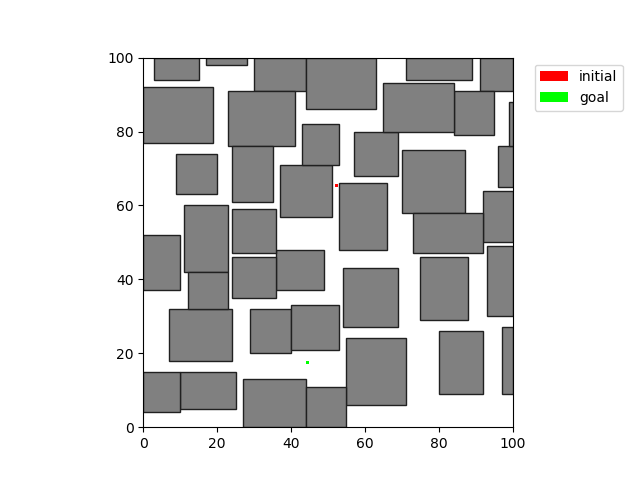
\includegraphics[scale=.40]{40_20_emp}
\caption{Domain}
\end{figure}

\begin{figure}[H]
\centering
	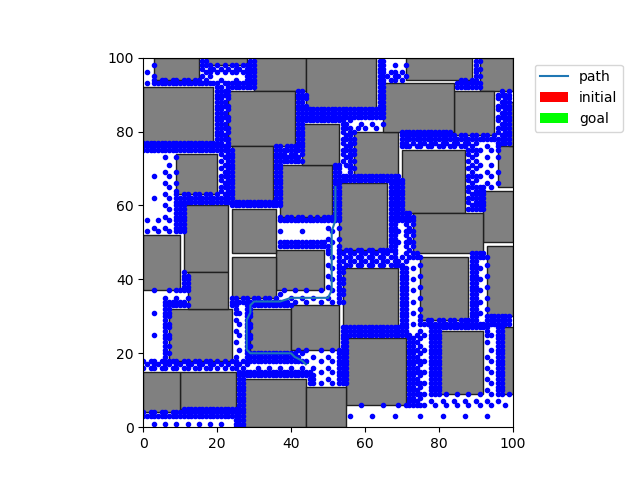
\includegraphics[scale=.40]{40_20_qtd_state}
    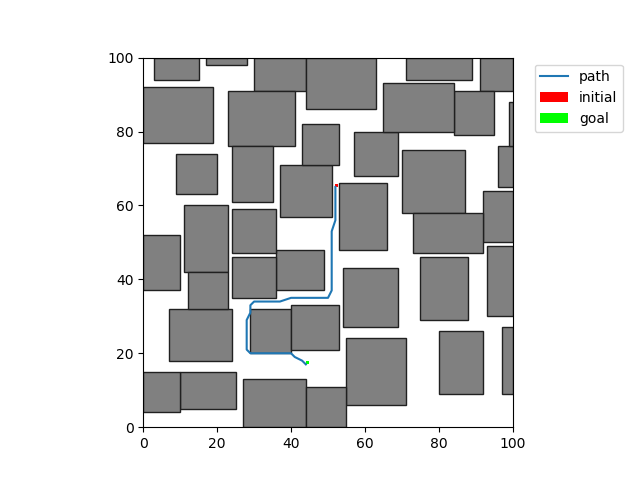
\includegraphics[scale=.40]{40_20_qtd_path}
\caption{QTD}
\end{figure}

\begin{figure}[H]
\centering
	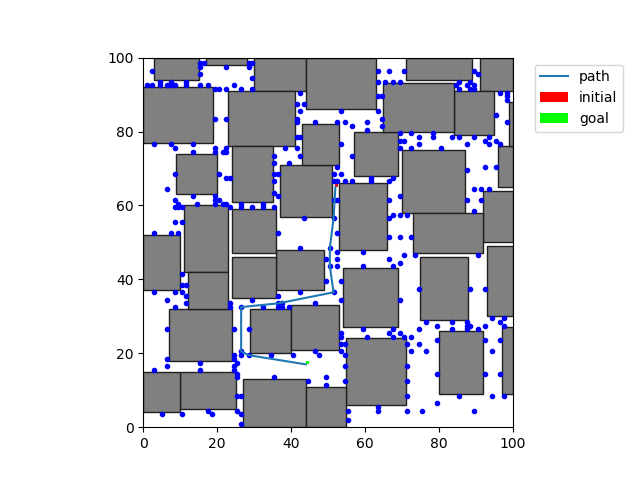
\includegraphics[scale=.40]{40_20_fbsp_state}
    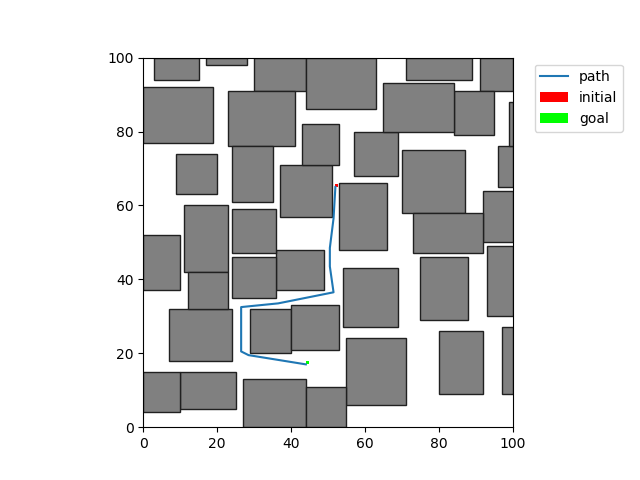
\includegraphics[scale=.40]{40_20_fbsp_path}
\caption{FBSP}
\end{figure}

\newpage

We ran the algorithm ten times on each domain type. The average results are in the table below:\\
\begin{center}
\begin{tabular}{ |p{2cm}||p{2cm}|p{2cm}|p{2cm}| p{2cm} | p{2cm} | }


 \hline
 \multicolumn{6}{|c|}{QTD} \\
 \hline
 number of obstacles/maximum size & total time & partition time & search time & total num nodes & num nodes in path\\
 \hline
 10/20 & 2.23   & 2.22  & 0.01  & 1134.10 & 17.20\\
 10/50 & 3.05   & 2.97  & 0.08  & 1303.90 & 26.60\\
 20/20 & 5.61   & 5.57  & 0.04  & 1809.50 & 27.70\\
 20/50 & 5.42   & 5.22  & 0.20   & 1655.70 & 40.10\\
 30/20 & 10.20   & 9.98 & 0.23  & 2252.60 & 36.20\\
 40/20 & 9.27  & 8.99 & 0.28 & 2140.90 & 53.50\\
 \hline
\end{tabular}
\end{center}

\begin{center}
\begin{tabular}{ |p{2cm}||p{2cm}|p{2cm}|p{2cm}| p{2cm} | p{2cm} | }

 \hline
 \multicolumn{6}{|c|}{FBSP} \\
 \hline
 number of obstacles/maximum size & total time & partition time & search time & total num nodes & num nodes in path\\
 \hline
 10/20 & 0.04   & 0.04  & 0.00  & 98.10 & 5.30\\
 10/50 & 0.04   & 0.04  & 0.00  & 83.50 & 5.40\\
 20/20 & 0.11   & 0.11  & 0.00  & 193.40 & 8.50\\
 20/50 & 0.09   & 0.09  & 0.00   & 155.30 & 8.00\\
 30/20 & 0.26   & 0.25 & 0.00  & 278.50 & 10.30\\
 40/20 & 0.29  & 0.29 & 0.01 & 303.10 & 13.20\\
 \hline
\end{tabular}
\end{center}

From these tables, several interpretations can
be made:
\begin{itemize}
\item
The size of the obstacles does not have much effect on 
either algorithm
\item
The number of obstacles has a large negative impact on 
the time for both algorithms
\item
For both algorims, the time it takes to find a solution is dominated by the time it takes to partition the state space
\item
Both the partition speed and the search speed is significantly faster for FBSP
\item
As expected, FBSP generates far fewer nodes

\end{itemize}

\subsection{Rapidly Exploring Random Tree (RRT)}

Below are figures of the solution found for different
domain types.\\

When the number of obstacles is 10:\\
\begin{figure}[H]
\centering

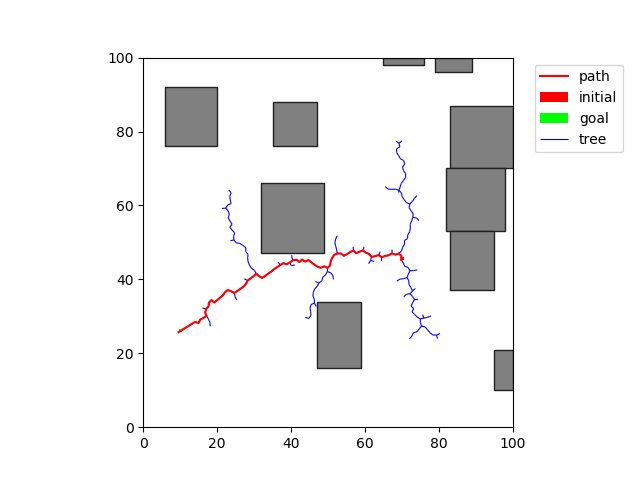
\includegraphics[scale=.40]{10_1.png}
\caption{10 obstacles, length,width$\sim$ uniform$(10,20)$}
% the runtime is: 0.3749270439147949 s
% the solver solved the problem!
% Number of nodes in the path:81
% Number of total nodes in the random tree:252
\end{figure}

When the number of obstacles is 10:\\
\begin{figure}[H]
\centering

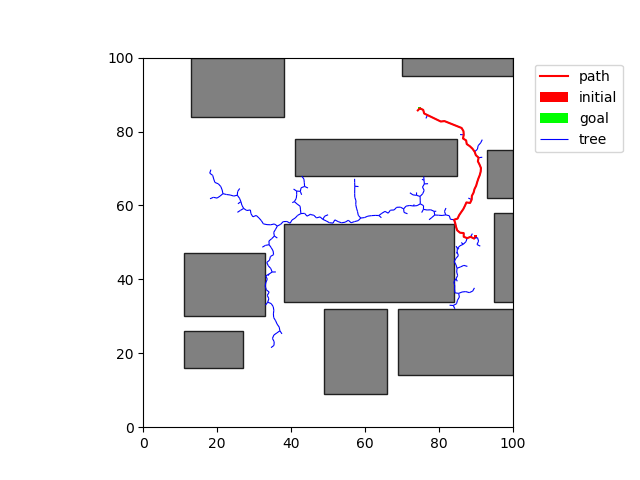
\includegraphics[scale=.40]{10_2.png}
\caption{10 obstacles, length,width$\sim$ uniform$(10,50)$}
% the runtime is: 0.8637630939483643 s
% the solver solved the problem!
% Number of nodes in the path:54
% Number of total nodes in the random tree:302
\end{figure}

When the number of obstacles is 20:
\begin{figure}[H]
\centering

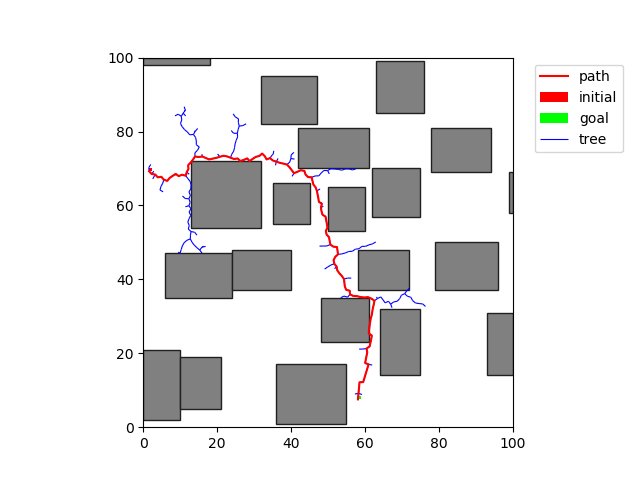
\includegraphics[scale=.45]{20.png}
\caption{20 obstacles, length,width$\sim$ uniform$(10,20)$}
% the runtime is: 0.8448247909545898 s
% the solver solved the problem!
% Number of nodes in the path:130
% Number of total nodes in the random tree:305
\end{figure}

When the number of obstacles is 20:
\begin{figure}[H]
\centering

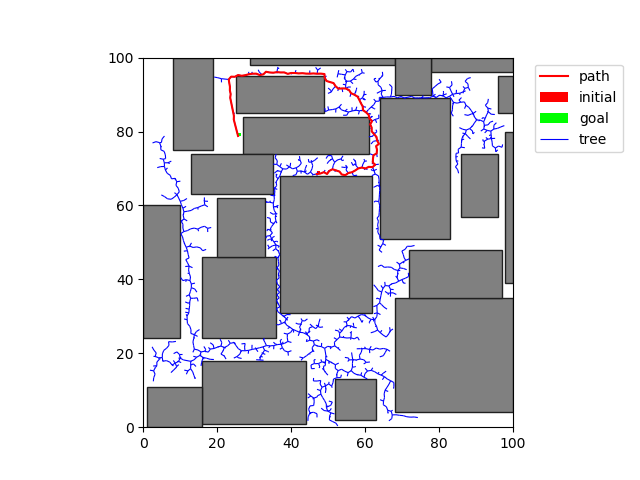
\includegraphics[scale=.45]{20_2.png}
\caption{20 obstacles, length,width$\sim$ uniform$(10,50)$}
% the runtime is: 14.890481948852539 s
% the solver solved the problem!
% Number of nodes in the path:96
% Number of total nodes in the random tree:1452
\end{figure}

When the number of obstacles is 30:
\begin{figure}[H]
\centering

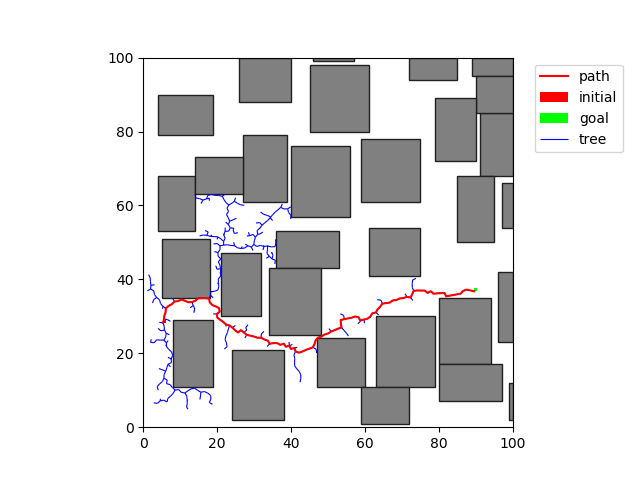
\includegraphics[scale=.45]{30.png}
\caption{30 obstacles}
% the runtime is: 2.2676401138305664 s
% the solver solved the problem!
% Number of nodes in the path:111
% Number of total nodes in the random tree:416
\end{figure}

When the number of obstacles is 40:
\begin{figure}[H]
\centering

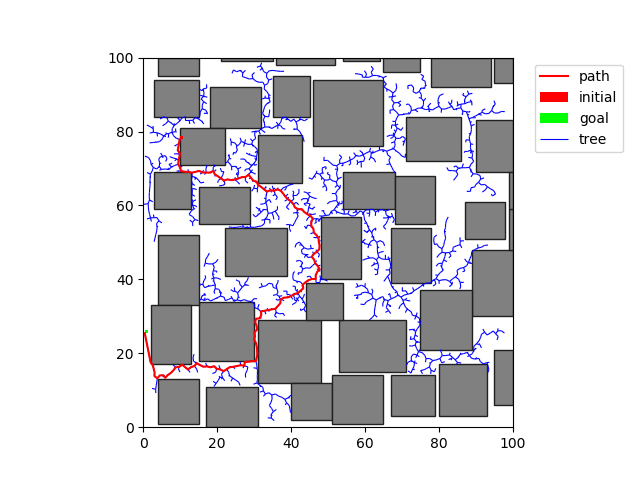
\includegraphics[scale=.45]{40.png}
\caption{40 obstacles}
% the runtime is: 26.552539825439453 s
% the solver solved the problem!
% Number of nodes in the path:152
% Number of total nodes in the random tree:1923
\end{figure}
When the number of obstacles is 45:
\begin{figure}[H]
\centering

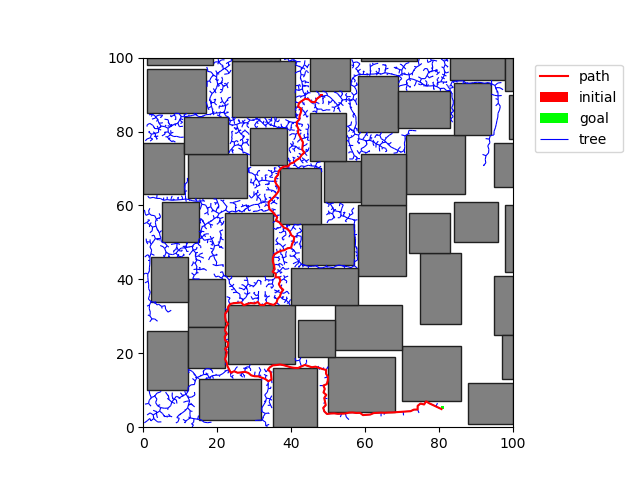
\includegraphics[scale=.45]{45.png}
\caption{45 obstacles}
% the runtime is: 26.552539825439453 s
% the solver solved the problem!
% Number of nodes in the path:152
% Number of total nodes in the random tree:1923
\end{figure}
When the number of obstacles is 45:
\begin{figure}[H]
\centering

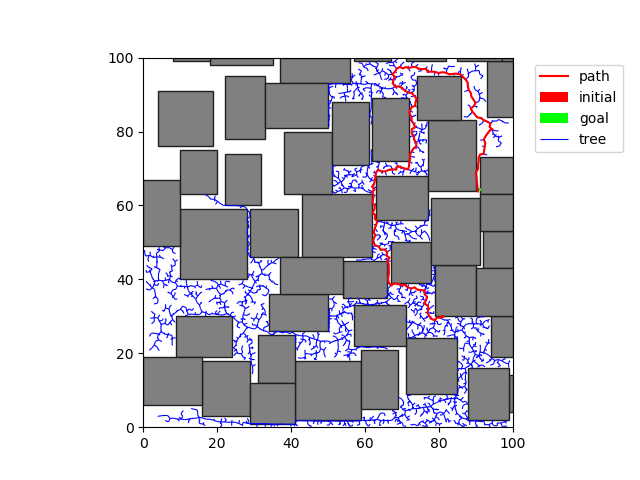
\includegraphics[scale=.45]{45_2.png}
\caption{45 obstacles}
% the runtime is: 26.552539825439453 s
% the solver solved the problem!
% Number of nodes in the path:152
% Number of total nodes in the random tree:1923
\end{figure}


We ran the algorithm ten times on each domain type. The average results are in the table below:\\
\begin{center}
\begin{tabular}{ |p{3cm}||p{3cm}|p{3cm}|p{3cm}|  }

 \hline
 \multicolumn{4}{|c|}{Experiment} \\
 \hline
 number of obstacles/maximum size& run time(avg) & num of nodes in the path(avg) & num of nodes in the tree(avg)\\
 \hline
 10/20   & 0.17    &45.25&   169.75\\
 10/50&   0.55425  & 87.25   &252.25\\
 20/20 &0.8525 & 91.5 &  333\\
 20/50    &5.979 & 98.25&  795\\
 30/20&  1.789  & 115.75 &414\\
 40/20& 20.715  & 136.75   &1459\\
 45/20& 57.59  & 167.67 &2511.33\\
 \hline
\end{tabular}
\end{center}

In summary, when the maximum size of obstacle is fixed, the run time and the number of nodes in the tree increase exponentially as the number of obstacles increases. The number of nodes in the path increases as the number of obstacles increases, but it is impacted less than the run time. On the other hand, when the number of obstacles is fixed, if we change the maximum size of obstacles, the rum time and the number of nodes in the tree increase in general.
Furthermore, if the number of obstacles is already large, then changing the maximum size will bring less impact to the behavior of the algorithm.
\end{document}
